\documentclass[letterpaper]{article}
\usepackage{natbib,alifexi}
\usepackage[english]{babel}
\usepackage{blindtext}
\usepackage{xcolor}
\usepackage{microtype}
\usepackage{amsmath}
\usepackage{listings}

\definecolor{dkgreen}{rgb}{0,0.6,0}
\definecolor{gray}{rgb}{0.5,0.5,0.5}
\definecolor{mauve}{rgb}{0.58,0,0.82}

\lstset{frame=none,
 language=Scala,
 aboveskip=3mm,
 belowskip=3mm,
 showstringspaces=false,
 columns=flexible,
 xleftmargin=.25in,
 basicstyle={\footnotesize \ttfamily},
 numbers=left,
 numberstyle=\tiny \color{black},
 keywordstyle=\color{blue},
 commentstyle=\color{dkgreen},
 stringstyle=\color{mauve},
 breaklines=true,
 breakatwhitespace=true,
 tabsize=3
}

\newcommand\todo[1]{\textcolor{orange}{Todo: #1}}

\title{Review: Accelerating Multi-agent Reinforcement Learning
with Dynamic Co-learning}
\author{Steve Homer$^1$, Fabian Perez$^1$, Quinten Rosseel$^1$ and Matthias Humt$^1$ \\
\mbox{}\\
$^1$\{steven.homer, fabian.perez, quinten.rosseel, matthias.humt\}@vub.be}


\begin{document}
\maketitle

\begin{abstract} \label{sec:abstract}
 This report reviews the paper from \cite{garant2015accelerating} which introduces a new approach to identify periodical experience transfer opportunities in large-scale, stochastic, homogeneous multi-agent systems (MAS) operating in a distributed manner. By using supervisory agents that compute and reason over high-level characterizations (contexts), similarities between agents are identified. Experiments show that the use of this method in the right settings can accelerate MAS learning significantly. We frame our understanding of the work and conclude with an empirical validation.
\end{abstract}

\section{Introduction} \label{sec:introduction}
In the standard Reinforcement Learning (RL) setting, an agent is placed into an unknown environment and provided with a set of actions from which it can choose. By performing an action, the agent can change its state which is then solely defined by the previous state the agent was in before and the chosen action. In certain states, defined by the problem setting, the environment provides feedback to the agent, often called \textit{reward} which can be either positive or negative. From this, the agent begins to approximate the underlying reward function in trying to maximize the expected future reward. Once having started to learn, the agent has to decide whether to exploit current knowledge by choosing the actions it expects to yield the highest reward or to explore new states with potentially higher rewards by trying new state-action combinations. This methodology is typically chosen, if the state-space is large and explicitly defining the correct actions to achieve the goal is either infeasible or even impossible as they are not known. An often cited example in this context is learning to ride a bike \citep{randlov1998learning}. The desired outcome is clear, but giving advice how to achieve it in terms of the correct movements to perform is quite difficult.

Multi-Agent Reinforcement Learning (MARL) is an extension to the standard RL problem setting, where multiple, often hundreds or thousands of autonomous agents try to pursue their individual goals simultaneously in a common environment. We speak of cooperative MARL, if multiple or all agents pursue the same goal, which means they try to maximize a common reward function. If they succeed, we say that they follow a (near-optimal) joint policy where policy means a mapping from states to actions. To achieve this however has proven to be difficult for large-scale multi-agent systems as it is computationally expensive and requires a large number of update steps until it converges.

An important insight on the path to solving this problem is the observation, that an exploitable structure in the problem setting--a distributed load balancing problem (Figure \ref{fig:loadbalancing}), where the agents try to share the work among each other as to minimize processing time--in the form of contextually similar groups of agents emerges during learning. Real world examples of this effect can be observed in \todo{Add examples}. Agents working on similar tasks under comparable environmental dynamics might benefit from sharing information to accelerate their individual learning progress which is the paradigm proposed in the paper under review. Additionally, strategies to identify promising candidates for information sharing and group formation are proposed, which will be introduced in the next section along with the test setup. In previous work, agents have either been trained individually on their local environment and neighbors, not being able to benefit from the experience of their peers, or as a hive, optimizing a single joint policy, which becomes quickly intractable even for a moderately large number of agents. But identifying contextually similar groups which are likely to greatly benefit from information sharing comes with its own difficulties. What information should be transferred? What does \textit{similar} mean? How well does this approach scale? Section \ref{sec:methods} will explore some of these questions in detail.
\begin{figure}[ht]
 \begin{center}
  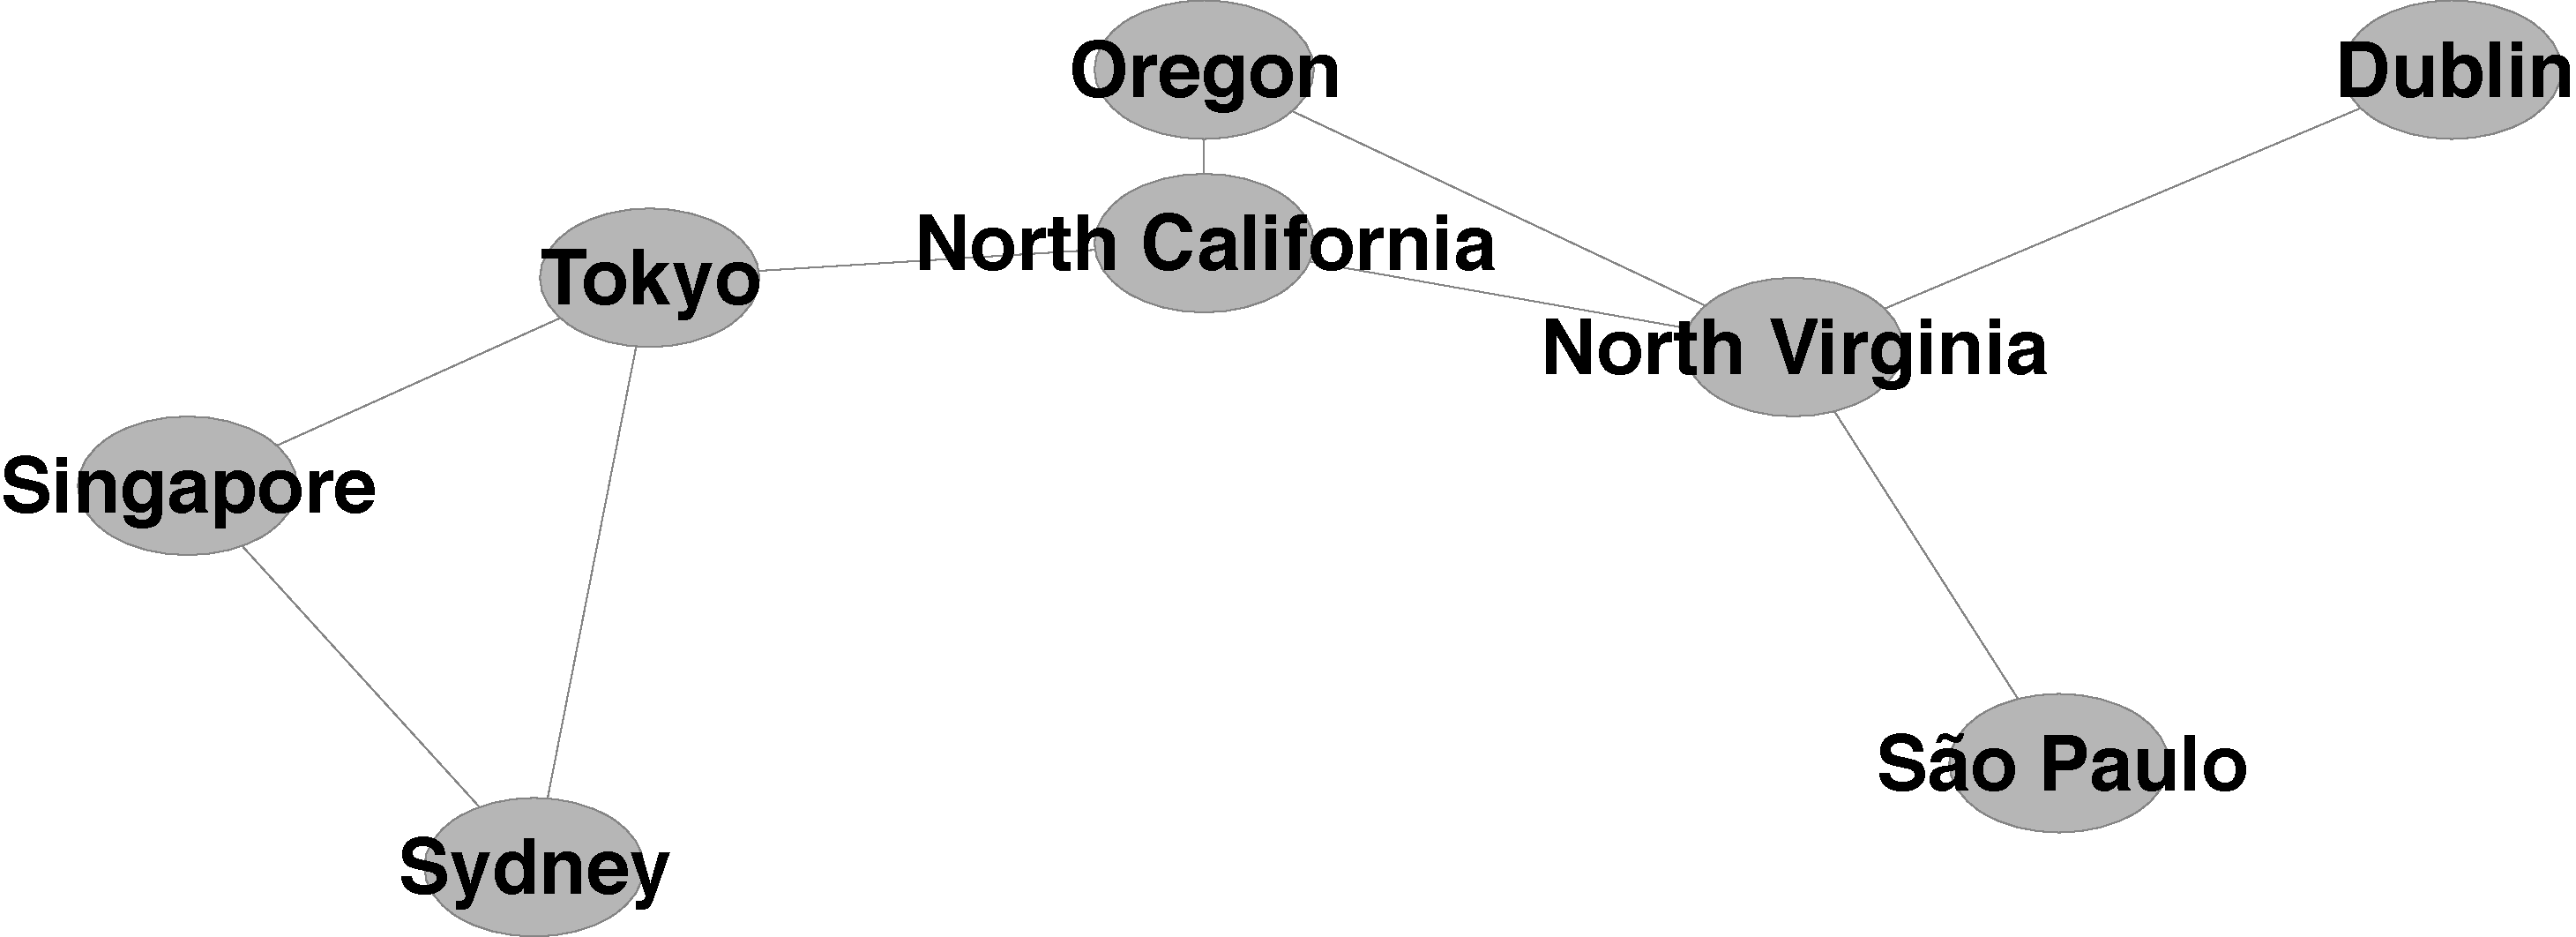
\includegraphics[width=\linewidth]{figures/loadbalancing}
  \caption{Small load balancing network \citep{garant2015accelerating}}
  \label{fig:loadbalancing}
 \end{center}
\end{figure}

\section{Methods} \label{sec:methods}
Several questions arise when designing a solution for this problem. I.e. How to identify groups in which information sharing is possible? What information should be transferred between agents in those groups? How can convergence in distributed and concurrent settings be guaranteed? This section provides a high level overview of the author’s conceptual framework and associates their scheme with our implementation of the model.  We highlight several design decisions and attempt to provide insights in difficulties and non-trivialities that pop up in the concretization process.

The authors propose a model of supervisor and subordinate agents. The subordinates can be seen as the domain specific workers of the system that aim to optimize a joint, domain-specific problem (e.g. load balancing distribution to minimise total service time). Supervisors keep track of subordinate groups and aim to accelerate the learning process using high level feature traits, collected from the subordinates.

The process starts by creating \textit{subordinate groups} (Figure \ref{fig:subordinate}) consisting of supervisors and subordinates. These groups remain fixed over the entire learning process. After groups are formed, supervisors periodically search for \textit{contextual compatible} subordinates in their subordinate group to compose experience \textit{sharing groups}. In these groups, subordinates are able to share learned experiences with any other member from the sharing group. Experience sharing between subordinates from different supervisors is not allowed. The contextual compatibility depends on factors like metric-defined interactions within a certain group of agents, also referred to as interaction sparsity in literature (e.g. $D^C$ distance measure in implementation) or aggregate effects over group interactions (e.g. amount of sent messages between agents over a time period).
\begin{figure}[ht]
 \begin{center}
  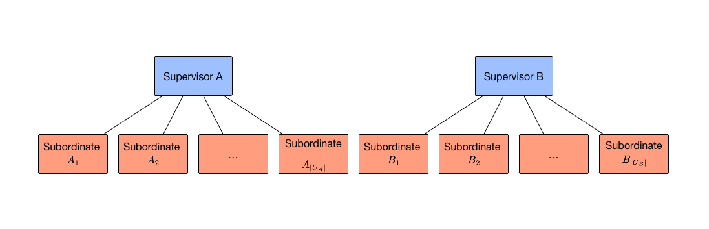
\includegraphics[width=\linewidth]{figures/subordinates}
  \caption{Supervisor hierarchy \citep{garant2015accelerating}}
  \label{fig:subordinate}
 \end{center}
\end{figure}
In order to keep the shared experiences concise, time-windows of $t$ timesteps are defined to characterize policy, reward and transition changes. Considering that decisions are framed as a Markov Decision Process (MDPs), experiences for one time window $[t_{0}, t_{e}]$ can be represented as a vector of tuples with $s_i, a_i, r_i$ and $s'_i$ corresponding to current state, action, reward and next state of the subordinate as depicted below. To be even more concise, another possibility would be experience merging within a given time window. This is disregarded due to increased complexity and information loss risks when states are not visited uniformly.
\begin{align*}
 \biggl<
  & (s_{i_{t_0}},a_{i_{t_0}},r_{i_{t_0}},s'_{i_{t_0}}), \\
  & (s_{i_{t_1}},a_{i_{t_1}},r_{i_{t_1}},s'_{i_{t_0}}), \\
  & \hdots                                              \\
  & (s_{i_{t_e}},a_{i_{t_e}},r_{i_{t_e}},s'_{i_{t_0}})
 \biggr>
\end{align*}
In a real word setting, experiences could be compressed by using linear regression equations, fitted to a variables set in the window. This is especially effective when agents infrequently change state. These \textit{compressed experiences} can be shared between subordinates using a supervisory agent as proxy. This allows the supervisor to derive context features from reported experiences and share it with subordinates that desire so. Though useful to save network bandwidth in a practical sense, from a theoretical point of view, compression is not desirable since it only adds complexity to the system. We chose to send raw, uncompressed experiences in order to update subordinate Q-values. The diagram below gives an overview of the model.
\begin{figure}[ht]
 \begin{center}
  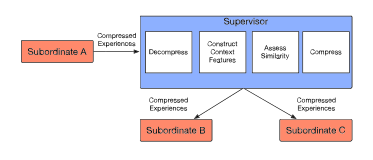
\includegraphics[width=\linewidth]{figures/diagram}
  \caption{Supervisory structure \citep{garant2015accelerating}}
  \label{fig:diagram}
 \end{center}
\end{figure}
To conclude the author’s theoretical framework we discuss how context features are constructed from the experiences that are passed along. We note that features like experience imbalance, policy divergence, unobservable state features and disjoint state visitations are attention points to take into account during context feature construction. More information on these concepts can be found in the paper. Since the Context Feature construction is domain-dependent, the authors only provide a general approach for doing so. The following paragraphs will explain our approach dealing with the proposed problem, but also ambiguities and missing information.

\subsubsection{Random Graph, Supervisory Topology, Task Allocation}
For each trial, a random network was generated for the given parameters of size and branching factor.  The supervisor topology was then imposed randomly on this network, differing from the original where the subordinate group of a supervisor was highly connected cluster.  Since the supervisor assignment was random, no assumptions could be made about the connectivity of other agents in the subordinate group.  In addition, the tasks were randomly allocated with random service time.  The goal of utilizing so much randomness in the construction of the simulations was to minimize design bias in the network and preclude any cross-domain assumptions that might creep in, especially in supervisor assignment.

\subsubsection{Worker Q-Learning with Softmax and Experience Integration}
Workers in the network improved their performance using a basic Q-learning algorithm with $\gamma = 0.1$ and a \textit{softmax} decision policy with $\tau = 0.1$.  Integrating experiences from other agents was done in a naive fashion, extracting the reward and neighbor index from the experience to update its corresponding Q-values for each shared experience.

\subsubsection{Distance Function}
The distance functions for each type of context feature followed a similar pattern that allowed for the proper interaction with the Boltzmann distribution used in the sharing selection algorithm.
(EQUATION)  :  $D^C(C1, C2) = round(0.1, e^-(abs(C1 - C2)))$
The quantized inverse exponential absolute difference produces discrete values that are near 1 when the distance is near 0 and and near zero when the distance grows large.  This allows the Boltzmann distribution to correctly weight small context feature distances with higher probabilities.

\subsubsection{Context Feature Construction}
Though stated in the paper that context feature construction is a transformation of an agent’s experiences for a given window into a vector or context features, it is only possible to create the context features only from the experiences of an agent by encapsulating all of the information relevant to the context features in the state of the agent. This sounds trivial, but in this case requires recording the local state (i.e. load, environment task allocation rate, and agent task allocation rate) of each of its neighbors into its own state.  Instead of encapsulating all of this data in this extended state, in our implementation the supervisor queries the agent and its neighbors for the information it requires and creates the context features from those responses.  These two methods are equivalent because the exact same information is gathered from querying as extracting from state.  This allowed us to have a simpler representation of state.

\subsubsection{COMPLAINING}
That being said, it shows that the choice of context features heavily influences the representation of the state of an agent.  For example here, an agent records information in its state that one would intuitively not think of as that agent’s state, like each of its neighbor’s loads and rates.  In multi-agent reinforcement learning, agents generally want to make decisions based solely on information gained from reward signals, in this case from other neighbors.  It seems odd then to need to record the internal state of those neighbors for the context features to be created solely rom experiences.  If you choose a more intuitive representation of state, i.e. information completely local to the agent, then creating the context features outlined in the paper is impossible. That is why the querying implementation was used here, because information required to create the context features could not be recovered from experiences alone without being extremely “generous” in what counts as the state of an agent..
\\\todo{More complaining after..?}

The problem stems from the fact that supervisor has no knowledge of the problem domain a priori, and therefore must extract all information from experiences. To see why it is impossible to extract context features from experiences alone, consider the following intuitive representation of an experience for the load-balancing problem, over a time window of size K:
\begin{lstlisting}
State(load, environmentRate, agentRate)
Process or Forward(i, agentID)
State’(load, environmentRate, agentRate)
InverseService(r)
\end{lstlisting}
\todo{Is this (above) what you wanted Steve?}\\
The supervisor can recover the neighbors of the agent by looking at where the agent has forwarded to this window.  That might not be all, or any, of its neighbors so we only recovered a subset of those neighbors.

If we allow the supervisor to look at other experiences in its memory of other agents (which the paper does not explicitly allow, but seems reasonable), then we can recover the relevant information from the experiences of the agents that are neighbors of the given agent, but only if those neighbors are in the supervisor’s memory.

Therefore, to get all of the information necessary to accurately calculate the context features for a given agent, that agent would have had to forward to all of its neighbors at least once in the window and those neighbors would also have had to be part of the same subordinate group (and then there’s still problems and the edges of the subordinate group).

Since this intuitive representation is untenable, we have to choose between using a bloated, unintuitive representation of state, or just querying the agents for the information we require.  We chose the latter.

\section{Results}
To present our results, we use the same methodology as the original paper to facilitate comparison.
\begin{figure}[ht]
 \begin{center}
  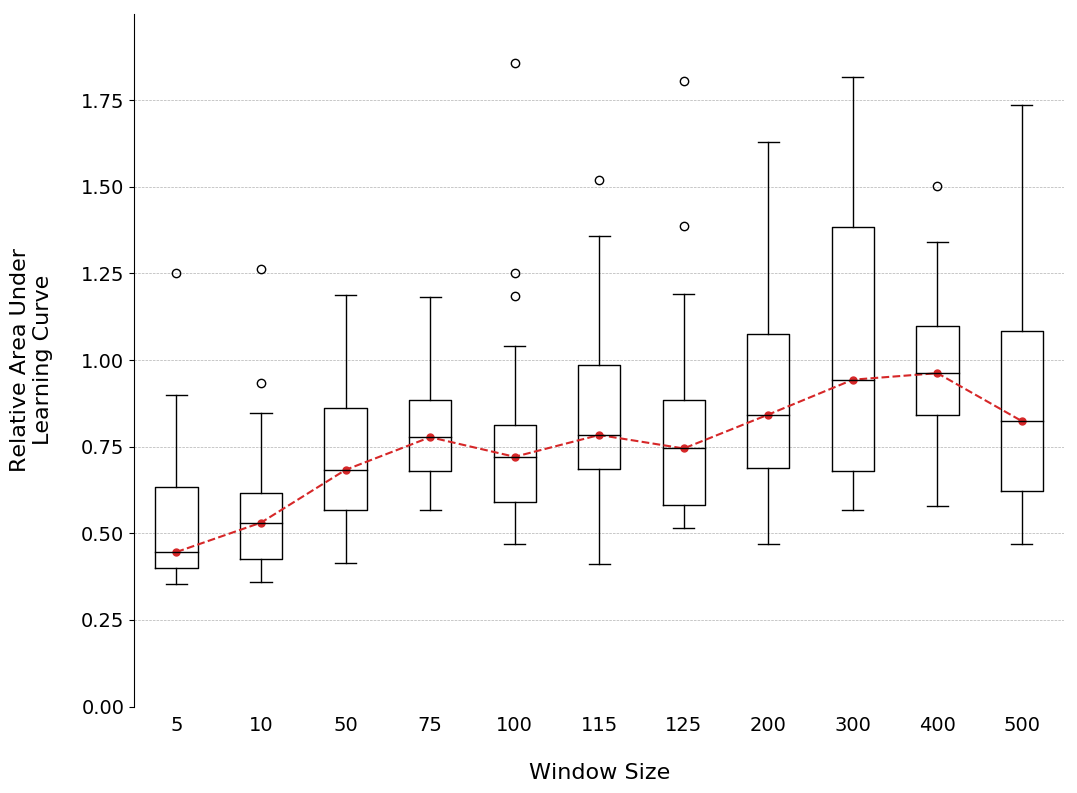
\includegraphics[width=\linewidth]{figures/figure4_extended}
  \caption{Effect of varying winow size K}
  \label{fig:windows}
 \end{center}
\end{figure}
\begin{figure}[ht]
 \begin{center}
  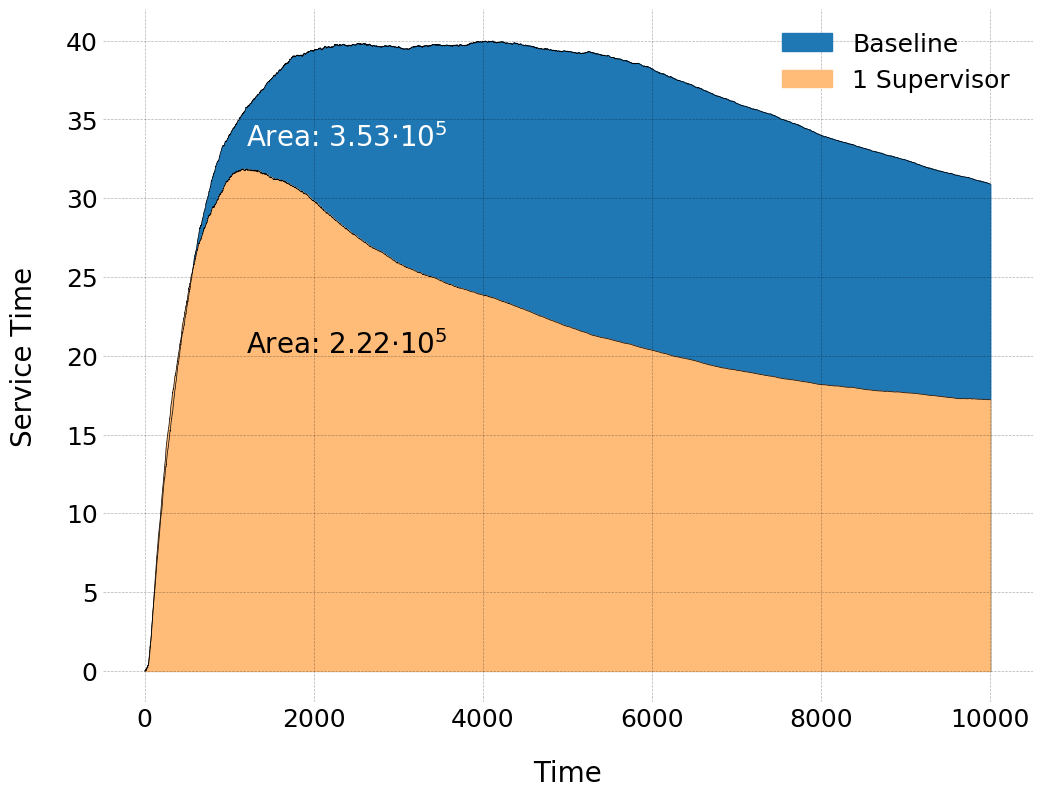
\includegraphics[width=\linewidth]{figures/figure5_light}
  \caption{Task Allocation Performance Evaluation}
  \label{fig:areas}
 \end{center}
\end{figure}
\begin{figure}[ht]
 \begin{center}
  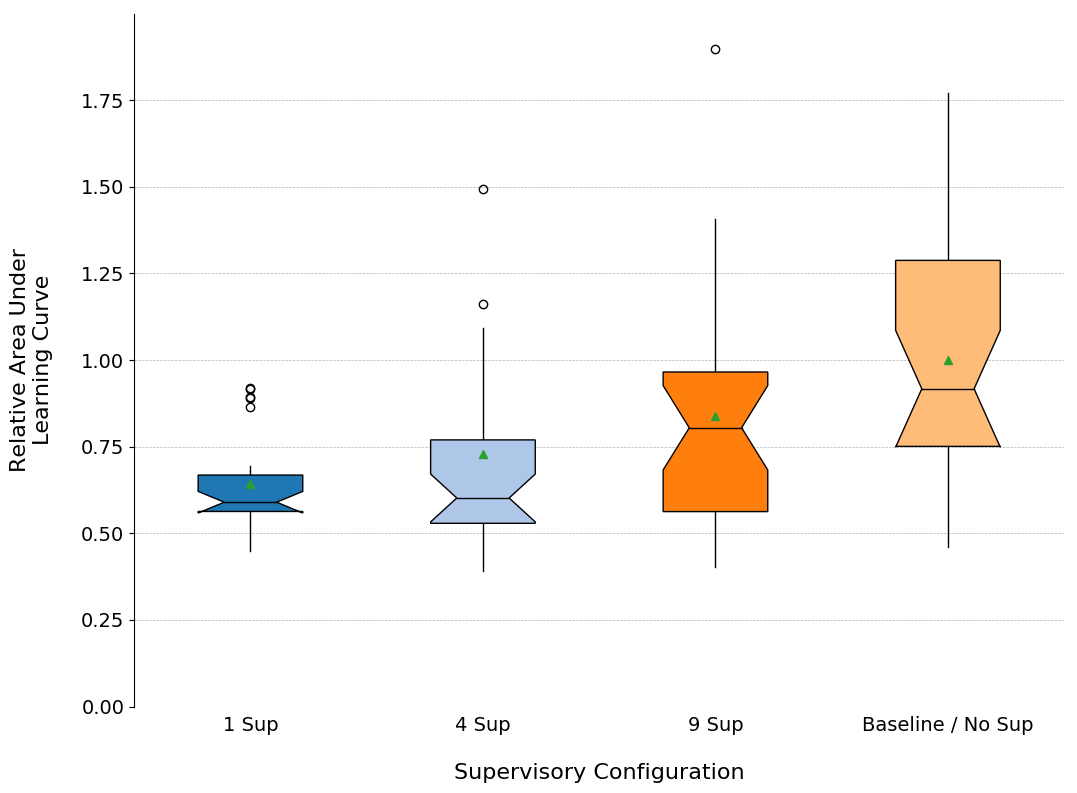
\includegraphics[width=\linewidth]{figures/figure7}
  \caption{Relative Performance by Supervisory Configuration}
  \label{fig:sups}
 \end{center}
\end{figure}
\begin{figure}[ht]
 \begin{center}
  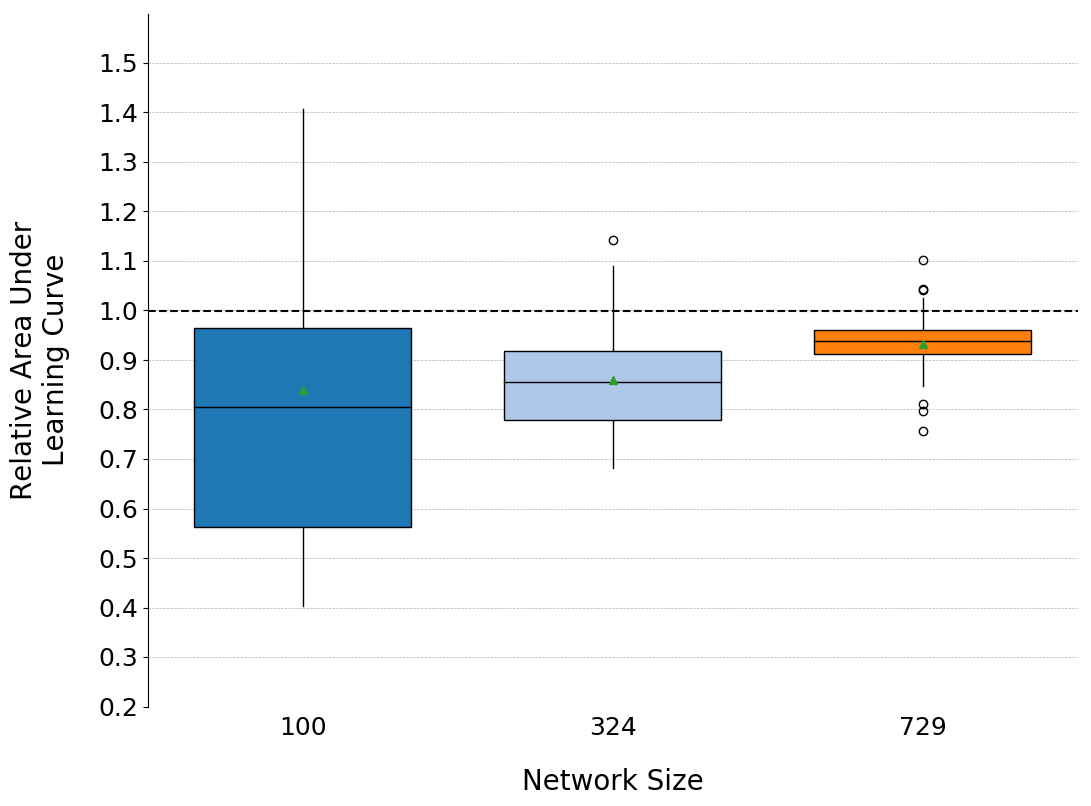
\includegraphics[width=\linewidth]{figures/figure8}
  \caption{Relative Performance as network size is varied}
  \label{fig:sizes}
 \end{center}
\end{figure}
\\\todo{Describe the performed simulations and their results}
\\\todo{Include chosen parameter settings}

\section{Discussion}
\todo{Summary and explanation of our work}

\section{Conclusion}
\todo{Add related work and an outlook}
\\\todo{Make sure all questions given below are answered}
\begin{enumerate}
 \item Does the introduction explain clearly the content of the paper
 \item whether there is sufficient background information to understand the relevance of the work
 \item whether the methods are clearly explained (can the results be reproduced?)
 \item whether the results answer the questions asked in the paper.
 \item whether all questions are answered
 \item whether the conclusion is sufficient
 \item and whether the overall style is ok and
 \item whether you believe things are missing in the discussion.
 \item etc.
 \item 3 positive points concerning the work, clearly specifying why you think they are well-
       done or interesting
 \item 3 negative points, which may include missing/unclear explanations or suggestions for
       improvement
 \item at least 3 clear and relevant questions on the content or the methods used which can be asked (next to other questions).
\end{enumerate}

\footnotesize
\bibliographystyle{apalike}
\bibliography{bibliography}

\end{document}
